\chapter{Introduction}
\label{chapter:introduction}
Every application that offers a method of interaction with a human being requires some form of user interface to enable this interaction. But what exactly characterises a user interface? The Oxford English Dictionary provides the following definition for "interface"\cite{inter87:online}:
\begin{displayquote}
\textbf{in\textperiodcentered ter\textperiodcentered face}, \textit{n.}: A means or place of interaction between two systems, organizations, etc.; a meeting-point or common ground between two parties, systems, or disciplines; also, interaction, liaison, dialogue.
\end{displayquote}

Thus, in the context of an application, a user interface is a means of interaction between the user and system based on common ground between these two entities. The common ground is a layer on top of the system which presents information from the system in a comprehensible manner to the user and translates user input to system-interpretable commands.

This is still a very abstract definition of what a user interface does. It does not specify how system information is presented, how the user provides input, what permissions and restrictions the interface must adhere to, et cetera. Nielsen\cite{nielsen1994usability} describes an overview of user interfaces throughout history which will provide some practical examples.

\textit{Batch systems} were one of the first user interfaces to be introduced. To interact with the system, a user submitted all of the system commands in one batch and had to wait for all of them to be processed before being presented with the results. It was a tedious and inconvenient way of interacting with systems, as erroneous commands would prevent the batch from successfully completing. Early batch systems also often required special operators to program the commands. Contemporary user interfaces generally still offer batch operation in some form or another, as its main advantage is that it can be used to perform menial tasks without continuous human supervision.

As the use of computers became more widespread, the \textit{line-oriented interface} was adopted as a method of interaction. The name is derived from the characteristic that the user interacted with a system on a single line; once submitted, the command could not be modified anymore. This characteristic enforces a use pattern where a dialog between the system and user takes place. The user answers questions posed by the system and issues commands with parameters. As long as the information is well structured this method of interaction still has valid use cases in present times, as it effectively delimits functionality, preventing novice users from running into issues.

The successor of line-oriented interfaces is the \textit{full-screen interface}. This interface aims to exploit a greater deal of the screen real estate by enabling the user to interact with more elements than just one input line, such as in the interface in figure~\ref{figure:fullscreeninterface}. The full-screen interface also introduced the concept of menus, where functionality available to the user is listed in a hierarchical structure. Menu design has been researched extensively\cite{paap1986optimal, landauer1985selection, fisher1990optimal} to determine the optimal balance of depth and breadth. Depth decreases complexity of menus while increasing ease of navigation; the contrary applies to breadth. Full-screen interfaces are still used present-day (e.g. electronic forms), albeit in adapted forms such as pop-up windows.

\begin{figure}
	\centering
	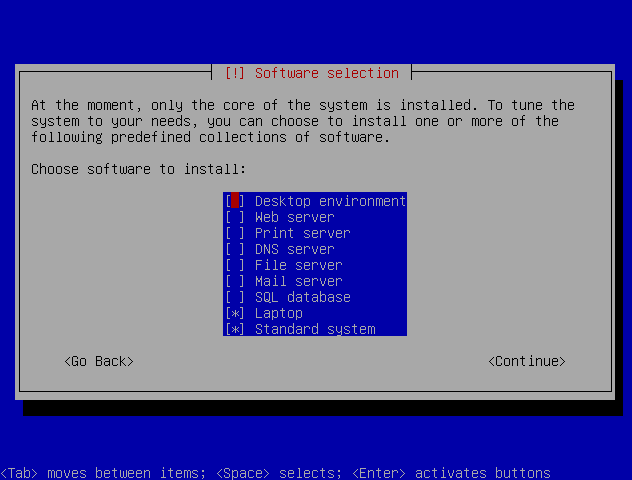
\includegraphics[scale=.5]{figures/debiannetinstall}
	\caption{A screenshot of Debian's full-screen interface during installation}
	\label{figure:fullscreeninterface}
\end{figure}

Finally, the user interface type which is currently the most widespread, is the \textit{\acrlong{gui}} (\acrshort{gui}). The vast majority of modern applications offer a graphical user interface as their primary method of interaction. A key characteristic of \acrshortpl{gui} is that interaction is offered through direct manipulation. Rather than issuing a command which exactly specifies those parameters of what has to happen, the user gets continuous feedback of their input commands. An example is resizing a window: if a user were to do this by a command, the dimensions are provided as parameters and the window resizes. In a \acrshort{gui}, the user can dynamically resize the window with the mouse. The obvious advantage of a \acrshort{gui} is that it can take advantage of the human sight to represent data in a more intuitive way. Research has shown that when the interface adheres to some fundamental principles, a user's cognitive performance increases with a \acrshort{gui}. An example of one of these principles is Miller's Law, proposed in his seminal research on information processing\cite{miller1956magical}. However, Nielsen also addresses the issue that motivates this research: a \acrshort{gui} sidelines the visually impaired from using an application.

Enabling the visually impaired to use applications despite a lack of or very bad vision has been an ongoing effort since \acrshortpl{gui} were widely accepted as the de facto standard\cite{boyd1990graphical}. However, it has proven to be difficult to design a \acrshort{gui} that is also accessible without visual cues. A big issue is that standardisation has proven ineffective: even though the United States has passed laws that enforce accessibility of websites\cite{Secti81:online} and the World Wide Web Consortium has developed the Web Content Accessibility Guidelines\cite{WebCo83:online}, research has shown that these guidelines are very often ignored and thus websites are rendered inaccessible for accessibility tools such as screenreaders\cite{leuthold2008beyond}.

This research aims to provide an alternative interface for visually impaired users for applications developed with the Apache Isis\cite{Apach60:online} framework. This interface will not serve as a replacement for the existing interface nor blend in with it. The interface is derived from the metamodel of the framework and thus content independent. This means that the interface is readily available for any Isis application and no alterations are necessary to add it to an existing application.

\section{Research questions}
\label{section:researchquestions}
The central research question in this thesis is:
\begin{displayquote}
\textit{Can a content independent graphical user interface be adapted to a non-visual interface so that visually impaired users are able to interact with the application?}
\end{displayquote}

For the non-visual interface to be useful it is imperative that it offers the same functionality as the graphical user interface. Therefore, we will also answer the following subquestion:
\begin{displayquote}
\textit{When implementing a non-visual interface, can the integrity of the domain model be maintained while providing an effective and simple method of interaction?}
\end{displayquote}

Finally, it is desired that the non-visual interface does not severely impact user performance, as this would imply that it is not a legitimate alternative to the existing interface. Thus, a second subquestion will be answered:
\begin{displayquote}
\textit{Compared to the standard interface, how is performance affected when the user employs the new interface?}
\end{displayquote}

\section{Overview of thesis}
\label{section:overviewofthesis}
A short overview of what this thesis will describe is given.